\begin{center}
\rotatebox{90}{
\scalebox{1.0}{
  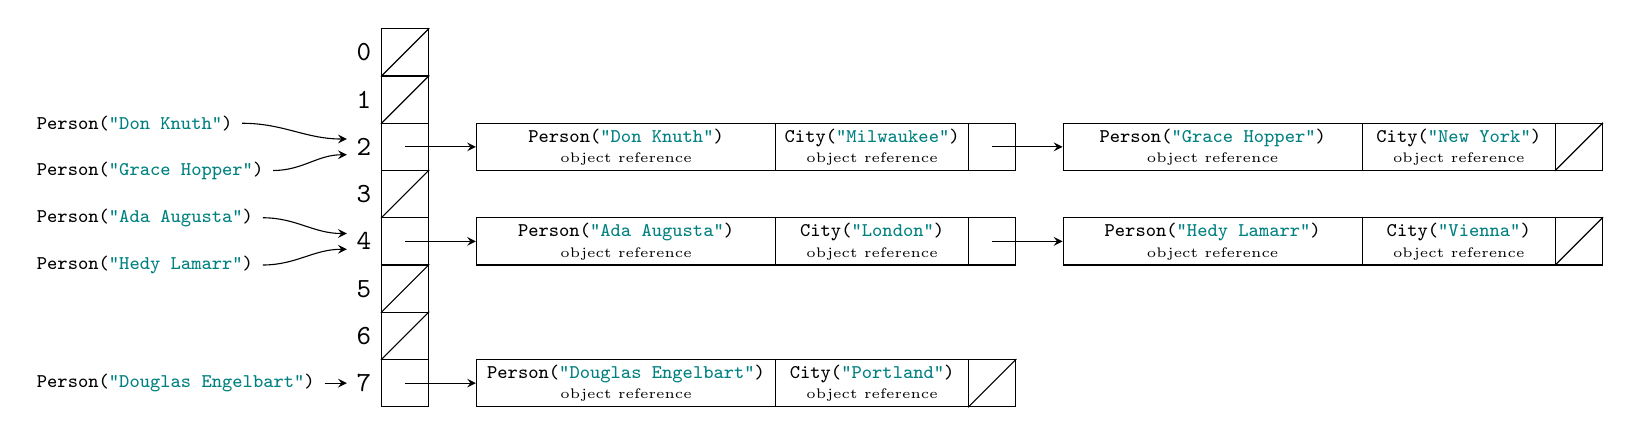
\begin{tikzpicture}[]
    \newcommand{\h}{6mm}
    \newcommand{\w}{6mm}
    \newcommand{\spacing}{(\w)}
    \newcommand{\Wspacing}{(8*\spacing)}
    \newcommand{\linkKeyWidth}{38mm}
    \newcommand{\linkValueWidth}{24.5mm}

    % args:
    % - 1: prefix
    % - 2: where
    % - 3: label
    \newcommand{\link}[4]{
      \coordinate (root) at (#2);
      \node[bucket,anchor=west, minimum width=\linkKeyWidth] (#1 key) at (root) {};
      \node[anchor=north] (#1 key label) at ([yshift=0.5mm]#1 key.north) {\scriptsize{#3}};
      \node[anchor=south] (#1 key type) at ([yshift=-0.5mm]#1 key.south) {\tiny{object reference}};
      \node[bucket,anchor=west, minimum width=\linkValueWidth] (#1 value) at ([xshift=\linkKeyWidth]root) {};
      \node[anchor=north] (#1 value label) at ([yshift=0.5mm]#1 value.north) {\scriptsize{#4}};
      \node[anchor=south] (#1 value type) at ([yshift=-0.5mm]#1 value.south) {\tiny{object reference}};
      \node[bucket,anchor=west] (#1 next) at ([xshift=\linkKeyWidth+\linkValueWidth]root) {};
    }
    
    \tikzstyle{null} = [draw=black]
    \tikzstyle{arrow} = [->,>=stealth, draw=black]
    
    \tikzstyle{key} = [
      rectangle,
      anchor=west,
      align=left,
    ]
    \tikzstyle{index} = [
      anchor=east,
      align=right,
    ]
    \tikzstyle{bucket} = [
      rectangle,
      draw=black,
      align=left,
      minimum height=\h,
      minimum width=\w,
    ]
    
    % keys
    \node[key] (knuth) at ({-\Wspacing}, {-1.5*\h}) {\scriptsize \texttt{Person(\textcolor{teal}{"Don Knuth"})}};
    \node[key] (hopper) at ({-\Wspacing}, {-2.5*\h}) {\scriptsize \texttt{Person(\textcolor{teal}{"Grace Hopper"})}};
    \node[key] (ada) at ({-\Wspacing}, {-3.5*\h}) {\scriptsize \texttt{Person(\textcolor{teal}{"Ada Augusta"})}};
    \node[key] (lamarr) at ({-\Wspacing}, {-4.5*\h}) {\scriptsize \texttt{Person(\textcolor{teal}{"Hedy Lamarr"})}};
    \node[key] (doug) at ({-\Wspacing}, {-7.0*\h}) {\scriptsize \texttt{Person(\textcolor{teal}{"Douglas Engelbart"})}};
    
    % buckets
    \node[bucket] (bucket0) at ( {0mm} , { 0*\h} ) {};
    \node[bucket] (bucket1) at ( {0mm} , {-1*\h} ) {};
    \node[bucket] (bucket2) at ( {0mm} , {-2*\h} ) {};
    \node[bucket] (bucket3) at ( {0mm} , {-3*\h} ) {};
    \node[bucket] (bucket4) at ( {0mm} , {-4*\h} ) {};
    \node[bucket] (bucket5) at ( {0mm} , {-5*\h} ) {};
    \node[bucket] (bucket6) at ( {0mm} , {-6*\h} ) {};
    \node[bucket] (bucket7) at ( {0mm} , {-7*\h} ) {};
    
    % indexes
    \node[index] (index0) at (bucket0.west) {\texttt{0}};
    \node[index] (index1) at (bucket1.west) {\texttt{1}};
    \node[index] (index2) at (bucket2.west) {\texttt{2}};
    \node[index] (index3) at (bucket3.west) {\texttt{3}};
    \node[index] (index4) at (bucket4.west) {\texttt{4}};
    \node[index] (index5) at (bucket5.west) {\texttt{5}};
    \node[index] (index6) at (bucket6.west) {\texttt{6}};
    \node[index] (index7) at (bucket7.west) {\texttt{7}};
    
    % links
    \link{first}{[xshift=\w/2+\spacing]bucket2}{\texttt{Person(\textcolor{teal}{"Don Knuth"})}}{\texttt{City(\textcolor{teal}{"Milwaukee"})}}
    \link{second}{[xshift=\w/2+\spacing]bucket4}{\texttt{Person(\textcolor{teal}{"Ada Augusta"})}}{\texttt{City(\textcolor{teal}{"London"})}}
    \link{third}{[xshift=\w/2+\spacing]bucket7}{\texttt{Person(\textcolor{teal}{"Douglas Engelbart"})}}{\texttt{City(\textcolor{teal}{"Portland"})}}
    \link{fourth}{[xshift=1.5*\w+2*\spacing+\linkKeyWidth+\linkValueWidth]bucket2}{\texttt{Person(\textcolor{teal}{"Grace Hopper"})}}{\texttt{City(\textcolor{teal}{"New York"})}}
    \link{fifth}{[xshift=1.5*\w+2*\spacing+\linkKeyWidth+\linkValueWidth]bucket4}{\texttt{Person(\textcolor{teal}{"Hedy Lamarr"})}}{\texttt{City(\textcolor{teal}{"Vienna"})}}
    
    % null values
    \draw[null] (bucket0.north east) -- (bucket0.south west);
    \draw[null] (bucket1.north east) -- (bucket1.south west);
    \draw[null] (bucket3.north east) -- (bucket3.south west);
    \draw[null] (bucket5.north east) -- (bucket5.south west);
    \draw[null] (bucket6.north east) -- (bucket6.south west);
    \draw[null] (fourth next.north east) -- (fourth next.south west);
    \draw[null] (fifth next.north east) -- (fifth next.south west);
    \draw[null] (third next.north east) -- (third next.south west);
    
    % pointers
    \draw[arrow] (bucket2.center) -- (first key);
    \draw[arrow] (bucket4.center) -- (second key);
    \draw[arrow] (bucket7.center) -- (third key);
    \draw[arrow] (first next.center) -- (fourth key);
    \draw[arrow] (second next.center) -- (fifth key);
    
    % hashing
    \draw[arrow] (knuth)  to[out=0,in=180] ([yshift= 1mm]index2.west);
    \draw[arrow] (hopper) to[out=0,in=180] ([yshift=-1mm]index2.west);
    \draw[arrow] (ada)    to[out=0,in=180] ([yshift= 1mm]index4.west);
    \draw[arrow] (lamarr) to[out=0,in=180] ([yshift=-1mm]index4.west);
    \draw[arrow] (doug)   to[out=0,in=180] ([yshift= 0mm]index7.west);
  \end{tikzpicture}
}
}
\end{center}
